\documentclass[]{article}

\usepackage{paralist} % Used for the compactitem environment which makes bullet points with less space between them

\usepackage{amsmath}
\usepackage{graphicx}
\graphicspath{ {pics/} }
\usepackage{algorithm}% http://ctan.org/pkg/algorithm
\usepackage{algpseudocode}% http://ctan.org/pkg/algorithmicx
\usepackage{multirow}
\usepackage{wrapfig}


\usepackage[a4paper, total={6in, 10in}]{geometry}



\usepackage{tabularx}
\newcolumntype{Y}{>{\centering\arraybackslash}X}

% ADD THE FOLLOWING COUPLE LINES INTO YOUR PREAMBLE
\let\OLDthebibliography\thebibliography
\renewcommand\thebibliography[1]{
    \OLDthebibliography{#1}
    \setlength{\parskip}{0pt}
\setlength{\itemsep}{0pt plus 0.3ex}
}

\usepackage[affil-it]{authblk} 
\usepackage{etoolbox}
\usepackage{lmodern}


\makeatletter
\patchcmd{\@maketitle}{\LARGE \@title}{\fontsize{16}{8}\selectfont\@title}{}{}
\makeatother

\renewcommand\Authfont{\fontsize{10}{8}\selectfont}
\renewcommand\Affilfont{\fontsize{7}{8}\itshape}



%----------------------------------------------------------------------------------------
%	TITLE SECTION
%----------------------------------------------------------------------------------------

\title{\vspace{-2.0cm}Towards Bayesian lifelong learning in mapping}


\author{Panagiotis Chatzichristodoulou, Rico  M\"{o}ockel, Kurt Driessens, Anne Van Rossum}
\affil{University of Maastricht, DoBots B.V.}


\date{}

%----------------------------------------------------------------------------------------

\begin{document}
\maketitle % Insert title

%----------------------------------------------------------------------------------------
%	ARTICLE CONTENTS
%----------------------------------------------------------------------------------------

\section{Introduction}

Simultaneous localization and mapping is one of the fundamental problems of autonomous systems\cite{probRobs}. In order for robots to be truly autonomous they have to be able to enter an environment and map its structure. To that direction, a lot of effort has been put in algorithms that are able to map static environments; with solutions like EKF-slam\cite{ekf} and FastSlam\cite{slam} we can now efficiently map such environments. 
The logical extension to methods that can map static environments is methods that remove this restriction. The idea of lifelong robot learning was introduced as a general concept to the literature by Sebastian Thrun\cite{liflonglearning}. Konolige et al.\cite{lifelongmaps} specifically focus on lifelong learning in mapping. In the PhD thesis of Walcott\cite{aishalong} long term mapping methods are decomposed to 4 basic subproblems: the problem of being able to continuously incorporate new information, tracking the growing DPG, detecting changes and update the map online, being able to handle changes to the map as changes occur with the passage of time.

The first two problems can be though of as compression problems as the map increases over time whereas the latter ones can be though of as dynamic environment problems. In this project the focus will be directed towards slam methods that use RGBD devices like Microsoft's Kinect to perform slam. The goal of this thesis is to introduce a novel approach to tackle the compression problem of long term mapping methods that use the Kinect devices while using Bayesian non parametric methods as the base of the solution.

Dirichlet processes and Dirichlet process mixture models\cite{nonParam} are the cornerstone of Bayesian non parametric statistics. The strength of those models lies in the fact that they allow the model's mixture components to grow as much as needed so as to best fit the data. The main motivation of this thesis is to integrate such methods to mapping algorithms as a means of creating compressed representations of the environment that also retain enough expressivenes so that they can be used as reference points when navigating through the environment. That would tackle the compression subproblem of long term mapping and would be a solid first step towards a general Bayesian solution to the long term mapping problem.

The rest of the paper is structured as follows. In Section \ref{sec:literature} relevant literature review will be reviewed, Section~\ref{sec:theory} will introduce the basic background theories of the model, Section~\ref{sec:model} will define the method presented in this paper, Section ~\ref{sec:results} will show experimental results of the method. Finally, conclusion and future directions are presented in Section ~\ref{sec:discussion}.
%------------------------------------------------

\section{Literature review}
\label{sec:literature}
Literature review will be focused on 4 related sub fields: Object based slam or semantic slam, point cloud object segmentation, non-parametric clustering methods ad the correspondence problem in slam.

\subsection{Object based slam}
Salas-Moreno et al.\cite{slam++} define a method of performing object based slam for specific classes of objects. The objects are identified by camera that is on top of the robot. By having a model of pre-trained objects, slam can be performed on environments where the robot knows what objects to expect. 
Castle et al. use object recognition to perform object based slam with the use of a hand-held cameras. Selvatici et al.\cite{objslam} use a similar approach while exploiting structural information such as object height and position within the room. That way a couch that is a large object situated in floor level is easier to be recognized.
Choudhary et al.\cite{objectpointslam} use point clouds and an object database to match objects currently seen with known objects within their database. They use omnimaper\cite{omnimaper} as their mapping method and as a representation a combination of the downsampled  voxel grids with additional normal and curvature information.  Finally, all their operations are done in the non-planar components of the point cloud.
Seongyong Koo et al.\cite{objectDisc} introduce a method of unsupervised object individuation from RGB-D image sequences. They cluster their initial cloud into candidate objects using Euclidean clustering and proceed to extract features like the Euclidean distance(L2) and the Kullback-Leibler distance between point cloud objects. They use IMFT to solve their tracking problem.

\subsection{Point Cloud Object clustering}

Trevor et al.\cite{pointSeg} take positional information, Euclidean distances and the normal of points to as input to their functions and output segments that are part of the same object. PCL library\cite{pcl} introduces methods like Euclidean clustering and conditional Euclidean clustering that use a number of heuristics that take normal as well as curvature information to extract segments in the point cloud that represent objects. Furthermore, a there is a lot of research on segmentation of point clouds in scenes, the emphasis is usually on extracting geometric primitives~\cite{planarSeg},\cite{planarSeg2} using cues like normals and curvature. Rabbani et al.\cite{segOverview} introduce a new method of object segmentation using KNN as their base algorithm. They also present a very informative literature review along with the strengths and weaknesses of existing methods. Finally Triebel et al.\cite{smartSeg} introduce a general clustering framework that does not rely on plane segmentation. Instead of segmenting the plane by using classical approaches like RANSAC or MLASAC they introduce a framework where they make no assumptions regarding plane data. 

\subsection{Non Parametric Bayesian methods}

Dirichlet processes and Dirichlet process mixture models are the cornerstone of Bayesian non-parametric statistics. Radford M. Neal\cite{bayes:neal} with his paper regarding MCMC methods for Dirichlet process mixture models made the definitive step towards Dirichlet process mixture models(DPMM's) receiving a lot of attention. Variational inference for DPMM's, introduced by Jordan et al.\cite{bayes:jordan} introduces deterministic tools to perform inference and approximate the posterior distribution and marginals of a dataset. Both methods have strengths and weaknesses and many tools have been established by using the two approaches as their base. Particle filter approaches of inference  have also been established with  Doucet et al.\cite{bayes:smc} introduce Sequential Monte Carlo as a fast way to approximate inference. For the purpose of this paper an SMC sampler will be defined in detail in the Model definition section.


\subsection{Correspondence}

Under the semantic slam context, correspondence refers to the problem of identifying objects as ones that have been encountered before during the mapping process. Towards that direction Cree et al.\cite{corresp:first} create a histogram of line segments of each landmark and compute their root mean square error. They then proceed to calculate their RGB signature to calculate the distance between different landmarks. Low et al.\cite{corres:sec} match Scale Invariant Feature Transform (SIFT) features, an approach which transforms image data into scale-invariant coordinates relative to local features. Lamon et al.\cite{corres:three} store a database of fingerprints which indicate the location in the robot's environment. The features are ordered and stored at a database at as they appear in the robot's immediate surroundings. A new fingerprint is computed for each new view and matched against existing ones. Finally, in Seghal et al.\cite{corres:four} an extension of SIFT descriptors to 3D data and point clouds is given.

\section{Theory background}
\label{sec:theory}

The basic theory background regarding the sampler will be presented in this section. Generalized Polya Urn is an extension on basic Urn\cite{caron} models for Dirichlet processes and serves as the base of the sampler presented in the theory section.

\subsection{Generalized Polya's Urn}

Dirichlet process priors have been widely used in the literature as non parametric Bayesian tools to estimate the number of clusters in the data\cite{antoniak}. Dependent dirichlet processes extend those tools by allowing the clusters in the data to vary with some variance over time by introducing dependencies on the data which can be temporal, positional etc. The DDPs are a natural extension of the DP's in domains where data cannot be considered exchangeable. The main motivation behind using such tools is that they can naturally be extended to dynamic environments to tackle the dynamic part of the long term slam problem.

A DDP also known as Generalized Polya Urn(GPU)\cite{caron} and has the property of randomly deleting partitions of clusters on every iteration. That way, it can cope with the variance of the data. The current notation defines the $n_{th}$ datapoint at time $t$,$x_{t,n}$ having an assignment $c_{t,n}$ at cluster $k \in \{1,2,..., K\} $. The size of cluster $k$ at time $t$ is defined as $s_t^k$. The GPU of this model at time $t$ can now be defined as:

\begin{algorithm}
    \caption{GPU}\label{GPU}
    \begin{algorithmic}[1]
        \Procedure{GPU}{$pointCloud, t$}

        \For{\texttt{$k = 1,...K_{t-1,N_{t-1}}$}}
        \State Draw $\Delta s_{t-1}^k \sim Binom(s_{t-1,N_{t-1}}^k, \rho) $ 
        \State Set $s_{t,0}^{k} = s_{t-1,N_{t-1}}^{k} -\Delta s_{t-1}^k$
        \EndFor
        \For{\texttt{$n = 1,...N_t$}}
        \State Draw $c_{t,n} \sim Cat( \frac{ s_{t,n-1}^{1} }{\alpha + \sum_k s_{t,n-1}^{k} }, \frac{ s_{t,n-1}^{K_{t,n-1}} }{\alpha + \sum_k s_{t,n-1}^{k} } , \frac{ \alpha}{\alpha + \sum_k s_{t,n-1}^{k} }) $
        \State If $c_{t,n} \leq K_{t,n-1}\ set:\ s_{t,n}^{c_t,n} = s_{t,n-1}^{c_t,n} + 1 , K_{t,n} = K_{t,n-1}$
        \State If $c_{t,n} > K_{t,n-1}\ set:\ s_{t,n}^{c_t,n} = 1 , K_{t,n} = K_{t,n-1} + 1$
        \EndFor
        \EndProcedure
    \end{algorithmic}
\end{algorithm}

Where Cat is a categorical distribution, Bin is the binomial distribution, $\alpha$ is the DP concentration parameter and $\rho$ is the deletion parameter of the GPU. This Generative Polya Urn distribution also has the shorthand notation GPU($\alpha,\rho$)

This process can be though of in the terms of a general chinese restaurant process\cite{antoniak} as shown in Fig.~\ref{generalPolya}. At time $t$, suppose there are $n$ customers seating at several tables in the restaurant. Each customer has to decide if he/she will remain at table with probability $p$ or leave the restaurant with probability $1-p$. Once all the customers make their decisions they leave the restaurant or remain seated (b). Each table occupied is moved according to the number of customers still seating in that table (c). A new customer then enters the table and either chooses to sit on one of the existing tables (e) or choose a new with probability proportional to the strength parameter $\alpha$ of the model(f).


\begin{wrapfigure}{l}{0.4\textwidth}
    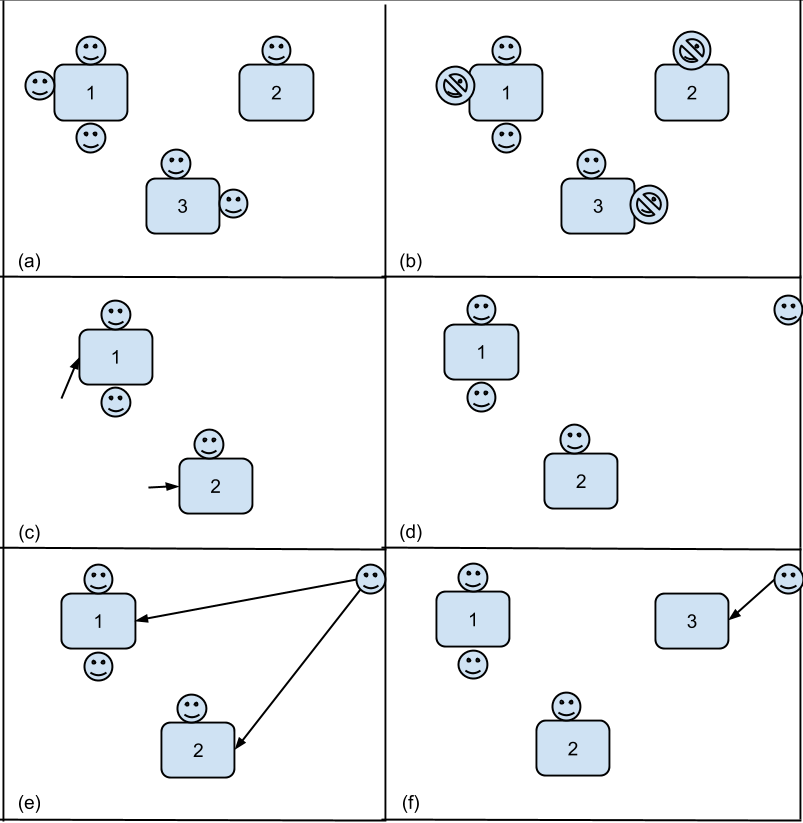
\includegraphics[width=0.9\linewidth]{generalPolya}
    \caption{General Polya}
    \label{generalPolya}
\end{wrapfigure}


\section{Model definition}
\label{sec:model}

\subsection{General pipeline}

The general flow of operations that occur in the EKF module is presented in Fig.~\ref{pipeline}. The slam module requests new observation readings given the cloud currently read by the sensors and the position of the robot. The pipeline takes that cloud, extracts clusters and returns the landmarks currently being observed while taking into account landmarks that where observed in the past. Landmarks and clusters are identical concepts representing a different layer in the pipeline. More specifically, clusters are output from the sampler from the sampler and are given as an input of landmarks to the EKF module.

\begin{wrapfigure}{l}{0.4\textwidth}
    \centering
    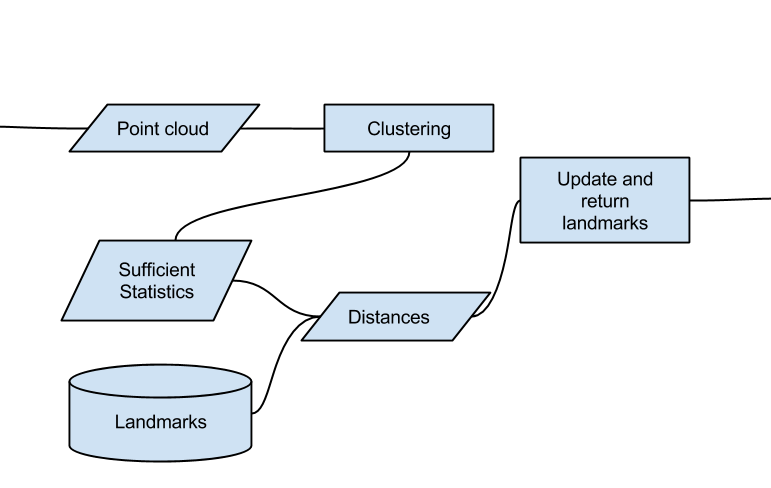
\includegraphics[width=.4\textwidth]{workflowSpec}
    \caption{Pipeline flow}
    \label{pipeline}
\end{wrapfigure}


\begin{algorithm}
    \caption{Landmark Layer}\label{euclid}
    \begin{algorithmic}[1]
        \Procedure{getLandmarkIds}{$pointCloud, timepoint, existingLandmarks$}
        \State $initialize(landMarkIds)$
        \State $pointCloudReduced \gets extractMetaFeatures(pointCloud)$ 
        \State $features \gets extractMetaFeatures(pointCloudReduced)$
        \State $landmarks \gets cluster(features)$  
        \For{\texttt{$landmarks$ as $landmark$}}
        \State $ (similarity, landId) \gets calcBestSim(landmark, existingLandmarks) $
        \If{$similarity >threshold$}
        \State $ addLandmarks(landMarkIds, landId)$
        \Else 
        \State $ newLandID \gets addLandmarkDB(landmarkDB, landmark)$
        \State $addLandmarks(newLandID)$
        \EndIf
        \EndFor
        \State \textbf{return} $ landMarkIds$\Comment{Return landmarks}
        \EndProcedure
    \end{algorithmic}
\end{algorithm}


\textbf{Method input:} The method takes as input a point cloud as it is currently being read by the kinect sensor.

\textbf{Lines 3-4:} The preprocessing the cloud is done in these steps. Feature extraction is done through the pcl\cite{pcl} library. A voxel grid is used to reduce the dataset size. A leaf size of approximately 3cm produces a good trade-off between precision and speed. The object representation used approach is similar to\cite{objectpointslam}. Instead of using the CSHOT descriptor, fpfh\cite{fpfh} histogram is used instead. A fast point feature histogram(fpfh) represents an angular signature between a point and its neighbors. The color signature of the cloud is being encoded with an approach similar to ~\cite{smcddp}. The color spectrum is discretized and what is extracted is the count of different color signatures between a point and its k nearest neighbors. Finally the position of every point is also given as input to the algorithm. The pipeline is presented in figure Fig.~\ref{pipeline}. The preprocessing outputs a vector of $\textbf{x} =(x_s, x_c, x_a)$ where $s$ represents the position information of the point, $c$ the color information of the point's neighbors and $a$ the angle information of the point's neighbors.

\textbf{Lines 5:} The clustering takes place in this line. The input of the method is the feature vector for every data point which is calculated in the previous steps. The clustering is done using the SMC sampler presented in the model definition section. 

\textbf{Lines 6-12:} The correspondence of previously seen landmarks to current observations is computed in lines 6-12. The calcBestSim function returns the landamrk with the highest similarity match with the landmarks already stored in the database.

\textbf{Lines 15:} The algorithm returns the list of the landmarks the robot sees in this current time.

Now that the basic theories are defined, the pipeline's components and its operating mechanisms can be presented in more detail.

\subsection{The sampler}

\subsubsection{The data distribution}
\label{data:dist}

Each point $x$ in the cloud is represented as a tuple $x =(x^s, x^a, x^c) $ where superscript $s$ represents spatial information, $a$ angle information, and $c$ color information. The method those features are extracted is explained in lines 3 and 4 in the general pipeline section. For the purpose of this project each point in the cloud is represented by vector of length 33 with the first three elements representing the space information, elements 4-6 angle information, and the rest color information.

The object model is a mixture of distributions over the data with each object being modeled as D($\theta_t^k$) where $\theta$ represents the parameters of object $k$ at time $t$. More specifically, each set \textbf{x} with $n$ datapoints at time $t$ is distributed as:
$$ x_{t,n} \sim D(\theta_t^k) = Normal(x_{t,n}^s| \mu_t, \Sigma_t) Mult(x_{t,n}^c | \delta_t) Exp(x_{t,n}^a | \lambda_t) $$

\begin{wrapfigure}{l}{0.25\textwidth}
    \centering
    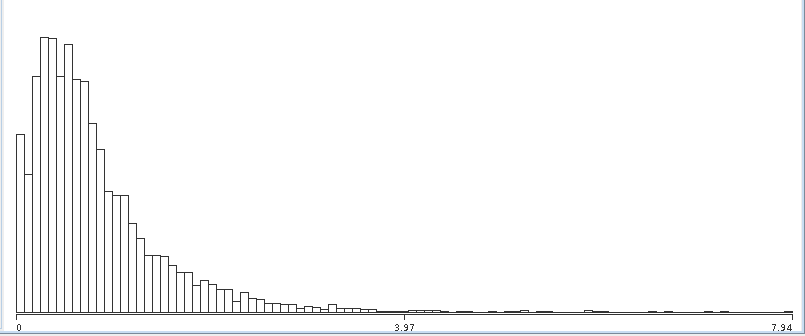
\includegraphics[width=.25\textwidth]{Kullback-Leibler}
    \caption{Exponential trend of distances}
    \label{pcl:kl}
\end{wrapfigure}

Where Normal is a three dimensional Gaussian distribution with mean $\mu$ and covariance $\Sigma$ representing the positional distribution of the data; Mult is a Categorical multinomial distribution with parameter vector $\delta$ representing the weights of the color distribution and Exp is an exponential with shape parameter $\lambda$ representing the angle distribution of the data within the cluster. The exponential distribution was chosen to model angular information after empiric evaluation showed that it would be a good fit for the angle signature distribution of the data as shown in Fig.~\ref{pcl:kl}.


Now that the distribution of the objects is defined, the progression of the sufficient statistics at time $t$ given $t-1$ given by:

$\theta_t^k | \theta_{t-1}^k \sim
\begin{cases} T (\theta_{t-1}^k) &\mbox{if } k \leq K_{t-1} \\
G_0 & \mbox{if } k > K_{t-1}. \end{cases}$

Where $T$ represents the transition kernel of the data given the previous state in the model. The case $ k > K_{t-1} $ represents the creation of a new cluster and $G_0$ is the base distribution of the DDP. In our case, the conjugate priors of the distributions of the data were chosen to model the base distribution. Therefore, $G_0$ is defined as:

$$ G_0(\theta_t^k)  = NiW( \mu_t^k, \Sigma_t^k | \kappa_0, \mu_0, \nu_0, \Lambda_0 ) Dir(\delta_t^k | q_0) Gam( \lambda_t^k | \alpha_0, \beta_0) $$

Where NiW is a Normal inverse Wishart distribution, Dir denotes a Dirichlet distribution, and Gam the Gamma distribution. $ \kappa_0, \mu_0, \nu_0, \Lambda_0, q_0,\alpha_0$ and $\beta_0$ are predefined parameters of the model. The generative process for the Dependent Dirichlet mixture model can be written for each timestep $t$ as:


\begin{compactitem}
\item Draw  $c_t$ $\sim$ $GPU(\alpha, \rho) $
\item $\forall$  k draw: $ \theta_t^k | \theta_{t-1}^k \sim
    \begin{cases} T (\theta_{t-1}^k) &\mbox{if } k \leq K_{t-1} \\
G_0 & \mbox{if } k > K_{t-1}. \end{cases}$
\item $\forall$  point $n$ draw $ x_{t,n} \sim F(\theta_t^{c_t,n})$
\end{compactitem}

Given the theory in \cite{caron}, the transition Kernel must satistfy:

$$ \int G_0(\theta_k) T(\theta_t^k | \theta_{t-1}^k) d\theta_{t-1}^k =  G_0(\theta_k) $$

The equation means that the invariant distribution must equal its base distribution. A typical way of meeting this restriction and forcing the sampler to converge to the original target density\cite{smc:theory} is to introduce a set of M auxiliary variables \textbf{z} such that:

$$ P(\theta_t^k | \theta_{t-1}^k) =  \int P(\theta_t^k | z_{t}^k)   P(z_t^k| \theta_{t-1}^k) dz_t^k $$

The transition kernel of the model can now be sampled by using the following formula

$\theta_t^k \sim T(\theta_{t-1}^k) = T_2 \circ T_1(\theta_{t-1}^k)$ with:
\begin{equation} \label{eq1}
    \begin{split}
        z_t^k  & \sim T_1(\theta_{t-1}^k)
        = Normal(\mu_{t-1}, \Sigma_{t-1}) Mult( \delta_{t-1}) Exp( \lambda_{t-1})\\
        \mu_t, \Sigma_t, \delta_t,  \lambda_t & \sim T_2(z_t^k)
        = NiW( \kappa_0, \mu_0, \nu_0, \Lambda_0 ) Dir(q_0) Gam(\alpha_0, \beta_0) 
    \end{split}
\end{equation}

where $\mu_t, \Sigma_t, \delta_t,  \lambda_t$  are posterior parameters given the auxiliary variables $z$.

\subsubsection{Sequential monte carlo sampler}

Sequential monte carlo samplers for Dirichlet process mixture models where introduced by Doucet et al~\cite{doucet} and serve as fast alternative to MCMC and VI methods of performing posterior inference. Given the previous definitions, the sampler is now defined as:


\begin{algorithm}[h]
    \caption{SMC for DDPM}\label{SMC}
    \begin{algorithmic}[1]
        \State \textbf{Input:} Points \{$x_{1,1:N_t}, ..x_{T,1:N_t}$\}with extracted features
        \State \textbf{Output:} Clusters representing of the data
        \For{$t = 1,...T$} 
        \For{$ l = 1,...L$} 
        \For{$ iter = 1,...S$} 
        \State Sample $(c_t)^{(l)} \sim Q_1$  
        \State Sample $(\theta^k ) \sim Q_2$
        \EndFor		
        \EndFor
        \For{$ k = 1,...K$} 
        \State Sample $\Delta s_{t-1}^k \sim Binom( (s_{t-1,N_{t-1}}^k)^{(l)}, \rho) $ 
        \State Set $s_{t,0}^{k} = s_{t-1,N_{t-1}}^{k} -\Delta s_{t-1}^k$
        \State Sample $( (z_{t+1}^k)^{(l)} ) \sim T_1((\theta_t^k))^{(l)} $
        \EndFor
        \State compute particle weights $w_t^l$
        \EndFor
        \State Normalize and resample weights
    \end{algorithmic}
\end{algorithm}

\subsubsection{Gibbs updates}
The proposal distribution $Q_1$ is the probability of an assignment $c_{t,n}$ given cluster sizes, parameters and concentration $\alpha$. Formally $Q_1$ can be written as:
\begin{equation} \label{Gibbs}
    Q_1(c_{t,n} | s_{t,n}^k, \theta_t^k, \alpha) \propto Cat( s_{t,n}^1,...s_{t,n}^K, \alpha ) \times
    \begin{cases} 
        F(x_{t,n} | \theta_t^{c_t} )  &\mbox{if } k \leq K_{t-1} \\
    \int P(x_{t,n} | \theta_t )G_0(\theta) d\theta & \mbox{if } k > K_{t-1}. \end{cases}
    \end{equation}
    Where $c_{t,n}$ represents cluster $c$ of point $n$ at time $t$, $s$ represents cluster sizes. The integral represents the posterior predictive distribution of the cluster times the base distribution with the parameters integrated out. A review of the literature helps understand how the posterior predictive formula is derived. More specifically, the analytic expression of the integral is:


    \begin{equation} \label{Q1}
        \begin{split}
            \int P(x_{t,n} | \theta_t )G_0(\theta) d\theta
            = t_{\nu_0-1}( x_{t,n}^s | \mu_0, \frac{\Lambda_0(\kappa_0+1)}{\kappa_0(\nu_0-1)}) \times \prod_{j=1}^V \frac{\Gamma(x_{t,n}^c)}{\Gamma(q_0)} \times \\ \frac{\Gamma(\sum_{j=1}^V q_0)}{\Gamma(\sum_{j=1}^V x_{t,n}^c)} \times Lomax(\alpha_0 + s_{t,n}^c, \beta_0 \sum_{j=1}^V x_{t,n}^c)
        \end{split}
    \end{equation}

    Where $t$ represents student's t-distribution with $\nu$ degrees of freedom, Lomax represents Lomax distribution with shape and scale, $\alpha$ and $\beta$ repsectively and the rest represent a Dirichlet-Multinomial(aka DirMul) distribution. The formulas of the posterior predictive distributions can be found in the literature with \cite{compendium} being a good example. 

    The conjugacy of the base and prior distribution allows for an easy sampling formula for proposal distribution $Q_2$ which is of the form: 

    \begin{equation} \label{Q_2}
        \begin{split}
            Q_2(\theta_t^k | \theta_{t-1}^k , x_t^k, z_t^k) \propto F( x_t^k | \theta_k) \times T_2(\theta_t^k | z_t^k) \\
            = NiW( \mu_t^k, \Sigma_t^k | \kappa_n, \mu_n, \nu_n, \Lambda_n ) Dir(\delta_t^k | q_n) Gam(\lambda_t^k | \alpha_n, \beta_n)
        \end{split}
    \end{equation}

    With:

    \begin{equation} \label{udpates}
        \begin{split}
            \kappa_n = \kappa_0 + N, 
            \nu_n = \nu_0 + N, 
            \mu_n = \frac{\kappa_0}{\kappa_0 + N} \mu_0 +  \frac{N}{\kappa_0 + N} \overline{x}^s\\
            \Lambda_n = \Lambda_0 + s_{x}^s,
            q_N = q_0 +  \sum_n x_i^c,
            \alpha_n = \alpha_0 +  N,
            \beta_n = \beta_0 +  \sum^n x_i^a\\
        \end{split}
    \end{equation}


    Where $\overline{x}$ defines the sample mean for the elements assigned at cluster $c$, $s_{x}$ the sample variance and $N$ denotes the number of observations. The formulas for the updates can be found at the literature of cojugate priors like\cite{compendium}.

    \subsubsection{Weight updates}

    The only thing left is to define the weight update step. More specifically, on every time step $t$ the weight of particle $l$ is calculated as:

    \begin{equation}
        w_t^{(l)} = \frac {P(c_t^{(l)} , \theta_t^{(l)}, x_t| 	\theta_{t-1} )}{P(c_t^{(l)} , \theta_t^{(l)}| 	\theta_{t-1} )}
    \end{equation}

    Using Bayes rule, the numerator can be written as:

    \begin{equation}
        P(x_t , | c_t^{(l)} , \theta_t^{(l)} \theta_{t-1} ) \times P(c_t^{(l)} , \theta_t^{(l)}|  \theta_{t-1} )
    \end{equation}

    Which can be calculated using equations $Q_2$ and $Q_1$ for the first and second part respectively. After the particle weights are normalized particles are drawn with probability proportional to their weights.

    \subsection{Decision Layer}

    The decision layer calculates how similar a cluster is to ones encountered before. To achieve that, distance measures must be defined between the stored clusters and the ones that are inferred at the current iteration of the algorithm. Distances between distributions are called divergences and a large amount of literature on divergences exists.

    Every cluster consists of a three part distribution as it was defined in section \ref{data:dist}. Now let $l$ be the distribution of a stored cluster and $o$ the distribution of a currently observed cluster. $l$ and $o$ can be decomposed into 3 parts: $l_G$,$l_C$,$l_E$ where G,C and E stand for Gaussian, Categorical and Exponential respectively. With that notation the distances between those distributions can be defined. For each individual landmark distribution $l$ and observation distribution $o$ the distances computed where the following: Wesserstein($l_G,o_G$), Kullback-Leibler($l_G,o_G$), SquaredHellinger($l_E,o_E$), Kullback-Leibler($l_E,o_E$), Kullback-Leibler($l_C,o_C$).

    The distance between every distribution can be transposed of a vector of length 5. That way, deciding if a cluster is part of a landmark that has been encountered before is now a problem of finding the optimal decision boundary given the distances at hand. For this project, the decision boundary by empiric evaluation of the landmarks.



    \subsection{Complexity}

    The complexity can be decomposed into three parts. The cloud downsampling, the clustering and the decision making process.
    $$
    O(total) = O(filter) + O(cluster) + O(decision)
    $$
    \textbf{Downsampling}: The complexity of the cloud downsampling pipeline can be decomposed to the one of its components. This means that the decomposed complexity is defined as follows:
    $$O(filter) = O(Downsampling + Stat\ Removal + RANSAC+ FPFH + Color\ estimation) $$

    Voxel downsampling searches for neighbors within a distance defined by the user and keeps an average value that equally represents the cloud. Since the operation involves searching for neighbors of a point, and since search operations take $O(log\ n)$ time where N is the number of points within the cloud, the complexity of voxelGrid downsampling is $O(k log n)$ where $k$ is the number of neighbors and $n$ the number of points in the cloud.
    Statistial outlier removal searches for k nearest neigbhors and removes those whose deviation is passed a certain threshold. Searching for k neighbors in cloud has a complexity of $O(k\ log\ n)$.A high amount of research has been done regarding the optimal complexity of RANSAC~\cite{RANSAC}. RANSAC has a complexity of $ O(k+ m_s*N)$ where k is the maximum amount of iterations defined by the user, $m_s$ the average number of models per sample $N$ the number of data points.
    FPFH operations have a complexity of $O(nk)$ as given in~\cite{fpfh}.
    Finally, for the operation of color estimation, the k nearest neighbors are chosen and some constant operation is performed on them. The complexity for color estimation then becomes $O(k\ log\ n)$ where $k$ is the number of neighbors, $n$ the number of points. 

    The downsampling pipeline has a total complexity of:
    \begin{equation} \label{Q_filt}
        O(filter) = O(k_{0}\ log\ n_{init} + k_{1}\ log\ n_{1} + k_{2}+ m_s*n_{2} + n_{3}k_{3} + k_{4}\ log\ n_{3} )
    \end{equation}

    Different $k$ indexes represent the number of neighbors defined for every operation. The $n$ represents the number of points used as input. Using the notation  of equation \ref{Q_filt}, $n_{init}$ defines the whole cloud, $n_1$ the cloud after operation 1, $n_2$ the cloud after operations 2 etc.

    \textbf{Clustering}: The complexity of the SMC sampler is defined in \cite{smcddp} as $O(TLKSN)$ where $T$ defines the time frames, $L$ the number of particles, $K$ the number of clusters, $S$ the number of samples, and $N$ the size of the dataset. 

    \textbf{Decision making}: The decision making takes $ O(\kappa * l^2) $ computational time where $\kappa$ defines the number of clusters output by the sampler and $l$ the number of landmarks currently stored in the database.

    The final complexity of the method can then be defined as:

    \begin{equation} \label{Complexity}
        O= O(k_{0}logn_{0} + k_{1}logn_{1} + k_{2}(t_M)+ m_s*n_{2} + n_{3}k_{3} + k_{4}logn_{3} + LKSn_3 + \kappa * l^2)
    \end{equation}

    \subsection{Landmark size}

    The basic block of this algorithm is a cluster containing an environment signature. In order to be able to compute how scalable the method is, the size of a single landmark will be computed. Each landmark is represented by a single row in an SQLite database. Each row consists of 32 real numbers and 1 auto increment integer. Given that SQLite databases assign the memory dynamically, the maximum amount of memory a cell can take will be calculated so that every other case is also included. According to the SQLite manual of datatypes a real value takes up to 8 bytes of memory. An auto increment integer takes up to 4 bytes of information, so the total number  of memory for a worst case scenario landmark is 260 bytes. This number can vary greatly over different environments and is a safe assumption to calculate the memory this method occupies.

    \section{Results}
    \label{sec:results}

    \subsection{Simple datasets}

    In this section the algorithm was tested against a simple dataset. Testing the method on simple datasets will make easier the extension to more complex clouds that will be used when mapping the environment. In order to test the sampling as well as the decision layer of the algorithm, a simple dataset provided by the pcl\cite{pcl} library was used. More specifically, a cloud consisting of two milk cartridges with different colors and poses where used. The initial cloud is shown in Fig.\ref{pcl:clust}(a). The cloud was given as input to the downsampling pipeline. The reduced cloud was then passed as input to the sampler and the clustering results are shown in Fig.\ref{pcl:clust}(b).

    \begin{wrapfigure}{l}{0.5\textwidth}
        \begin{tabular}{c}
            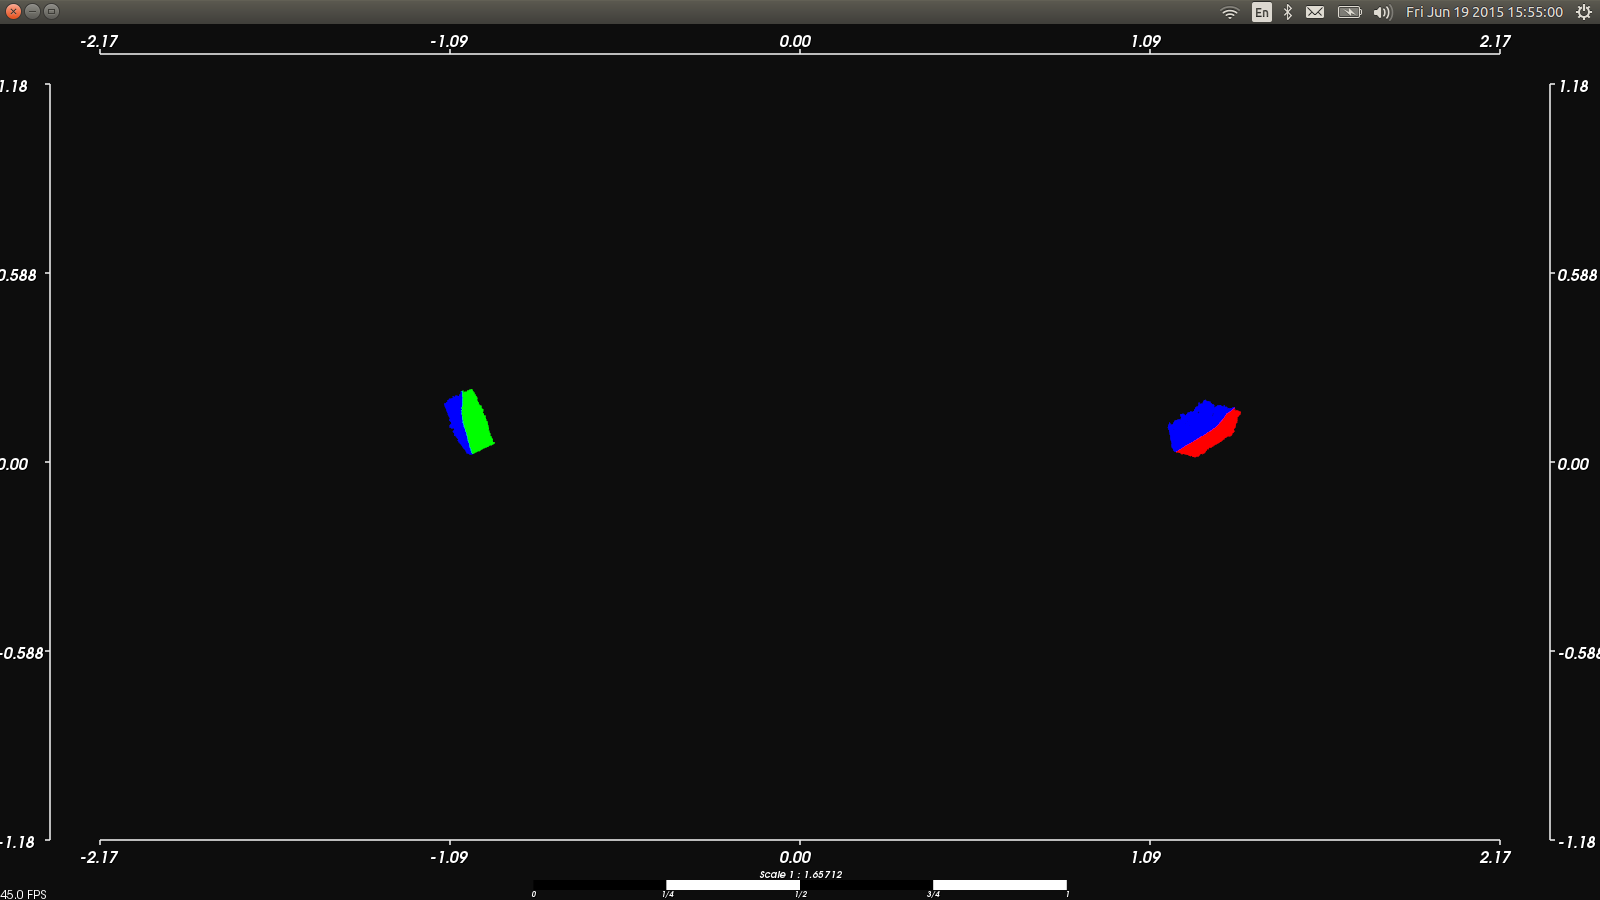
\includegraphics[width=.4\textwidth]{clusterings/coloursSource} \\
            (a) Raw cloud  \\
            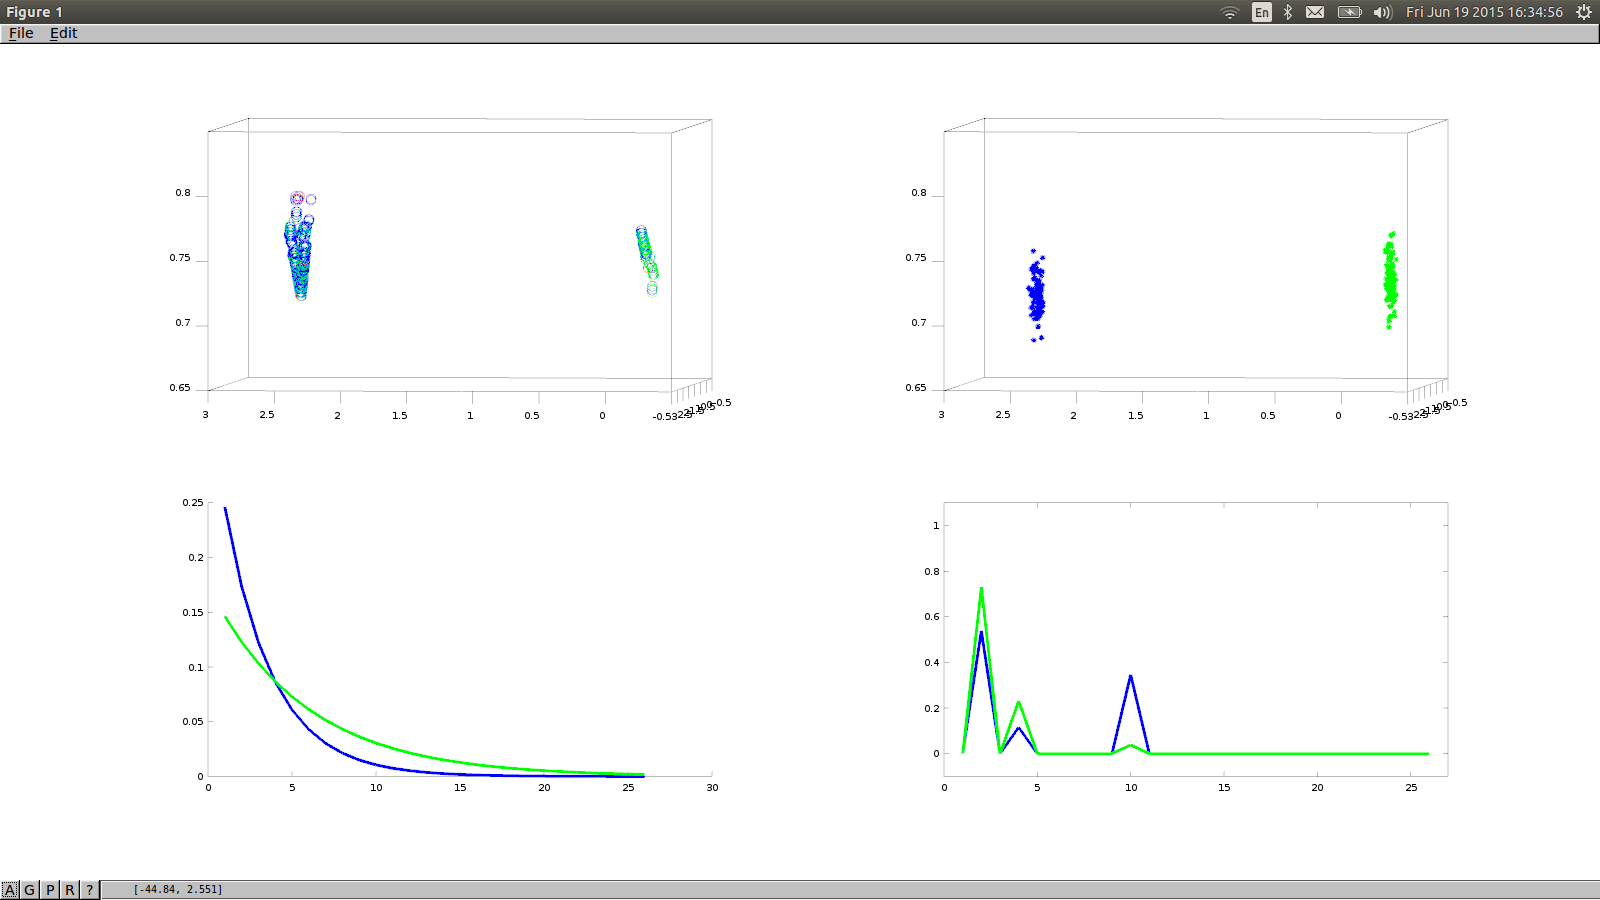
\includegraphics[width=.4\textwidth]{clusterings/coloursCorrect} \\
            (b) Post clustering \\[6pt]
        \end{tabular}
        \label{pcl:clust}
    \end{wrapfigure}

    More specifically, the reduced point cloud is shown in the top left part. It is significantly smaller in size and this cloud along with all the meta-information needed to perform the clustering are given as input to the sampler. The sampler outputs a mixture of distributions that best fits the input data. The clustering output is shown in Fig.\ref{pcl:clust}(b) with the top right being the Gaussian distributions inferred, bottom left the exponential and bottom right the categorical representing the color information of the cloud. The height of the objects leads to distribution with high variance in the z axis. The sampler outputs 2 clusters for the data with each box being assigned separately. The color signature each cluster carries is correctly captured in the bottom right part of Fig.\ref{pcl:clust}(b). The two boxes are similar in size but their orientation is different and this slight difference is shown in the exponential part of the signature. Each box is now captured as an environment signature that consists of a Gaussian, a Categorical, and an Exponential part.


    \begin{center}
        \begin{tabularx}{1.01\textwidth}{|c *{6}{|Y}|}
            \hline
            \multicolumn{6}{|l|}{\centerline{UUID 1}} \\
            \hline LandUUID & GausKL & GausWes & ExpHel & ExpHel & CatKL \\
            \hline
            1&0&1.18111e-07&0&0.164045&0 \\
            \hline
            2&13.5579&22449.9&1.56956&0.376699&13.8155 \\
            \hline
        \end{tabularx}    
        \label{dist}
    \end{center}

    Table~\ref{dist} shows the distances between every cluster computed against the first. The Gaussian counterparts of the clusters have significant distances due to the distance every cluster has in space. On the other hand, the Distances between their Exponential parts are not that large and the overlap between the categorical singatures leads to medium distances in their Categorical counterparts. Those distances are the information that is being passed to the decision layer to match existing landmarks with new ones. 

    \subsection{Expresiveness and decision layer}

    Post clustering, of operations in the pipeline have to do the comparison of clusters currently extracted with landmarks already stored in the database. The accuracy of the operations is dependent on the expressiveness of the signatures the clusters carry and this is displayed in the examples presented in Fig.\ref{pip:bounds}. The decision boundary of the pipeline can be decomposed into three basic parts; a positional, a color and an angular boundary. Fig.\ref{pip:bounds} shows the behavior of the decision layer with respect to the Gaussian(positional) and Categorical(color) parts. 

    \begin{wrapfigure}{l}{0.65\textwidth}
        \begin{tabular}{cc}
            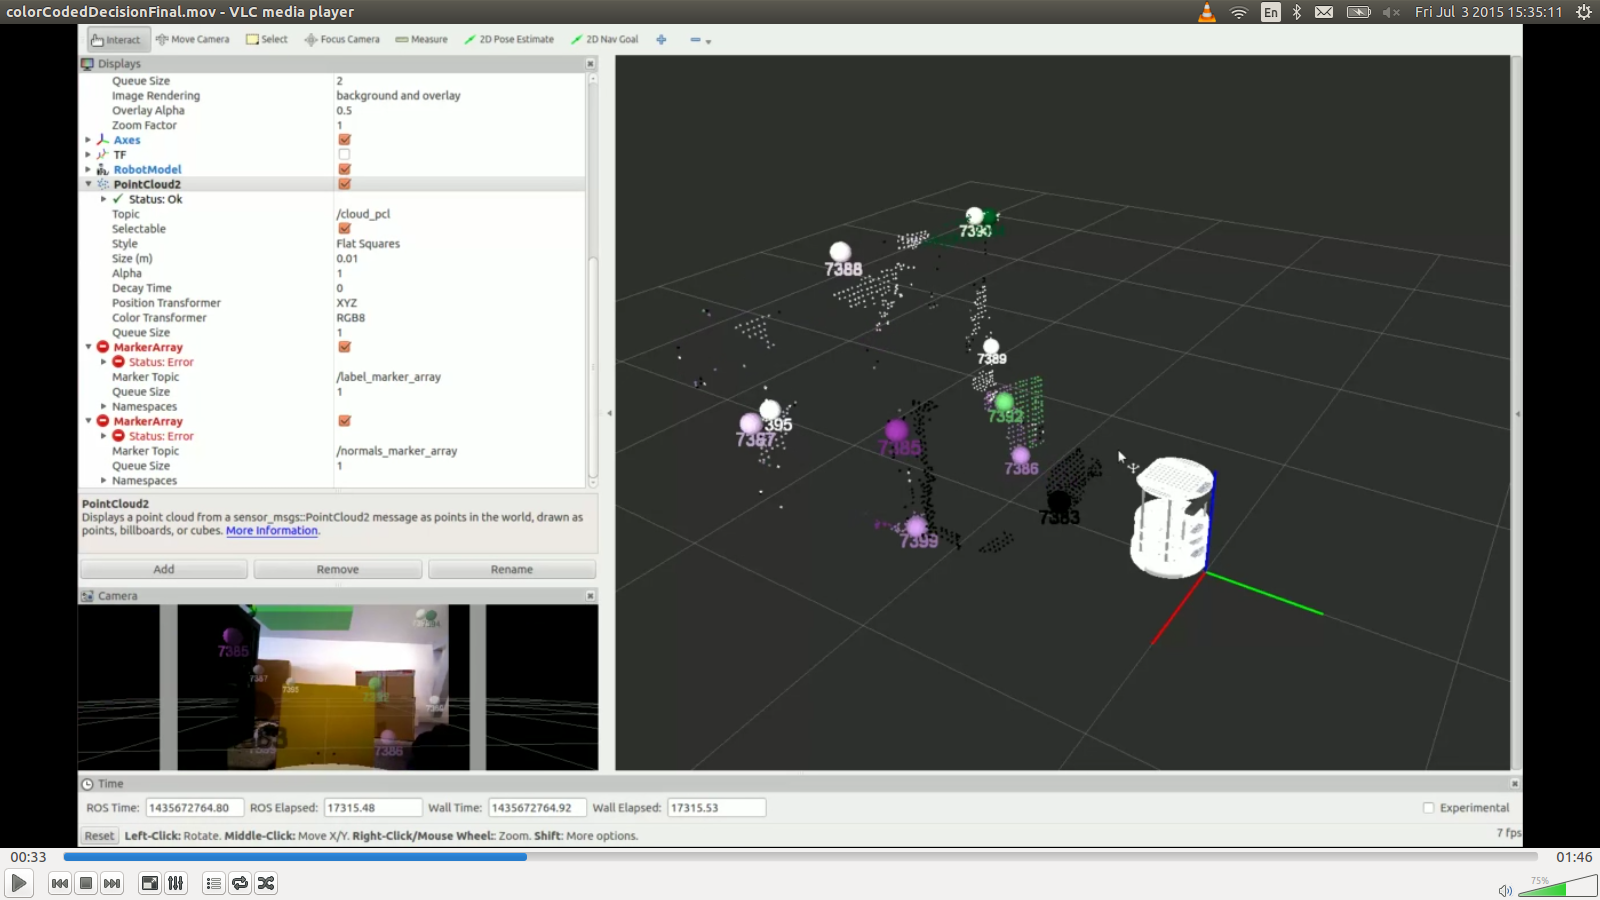
\includegraphics[width=.3\textwidth]{colorBound} &   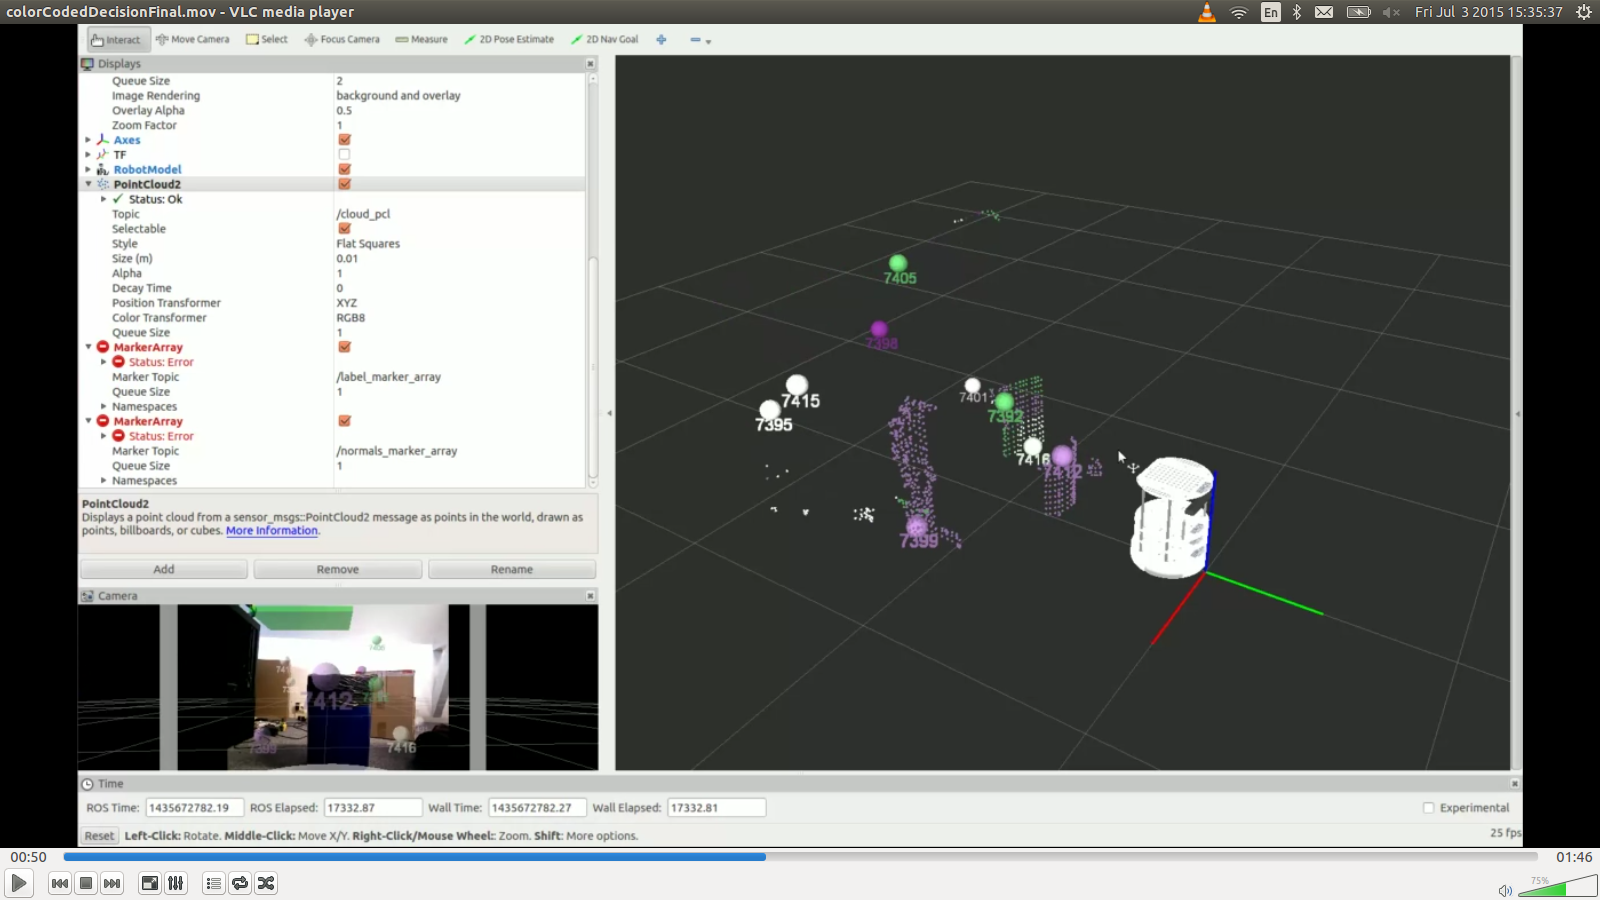
\includegraphics[width=.3\textwidth]{colorBound2} \\
            (a) Yellow Folder& (b) Blue trashcan \\[6pt]
            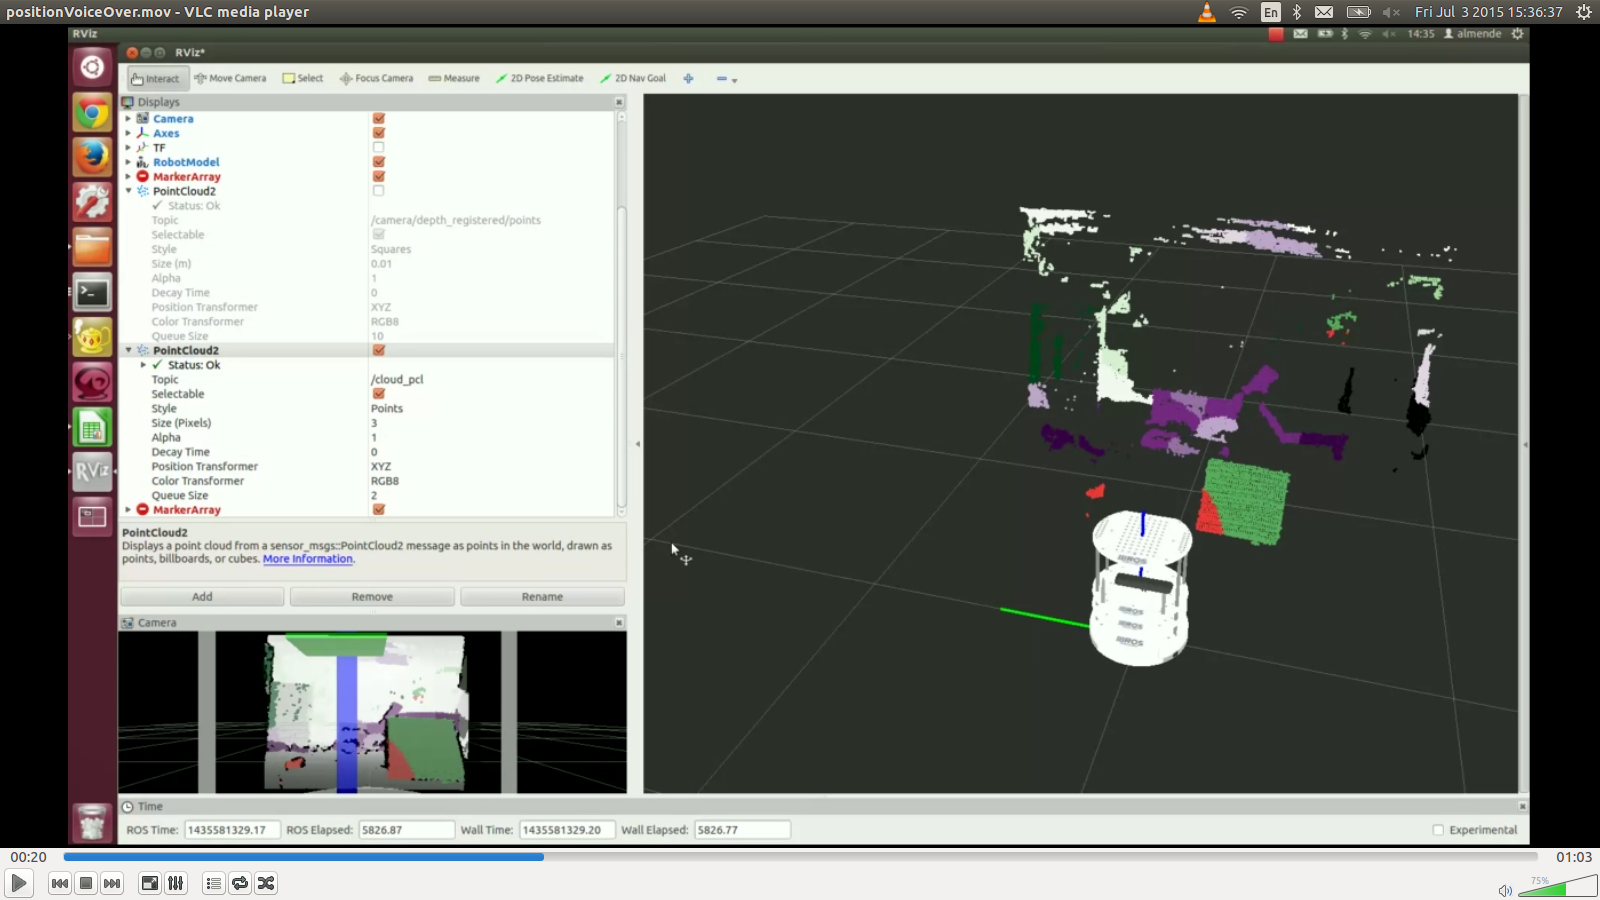
\includegraphics[width=.3\textwidth]{posBound} &   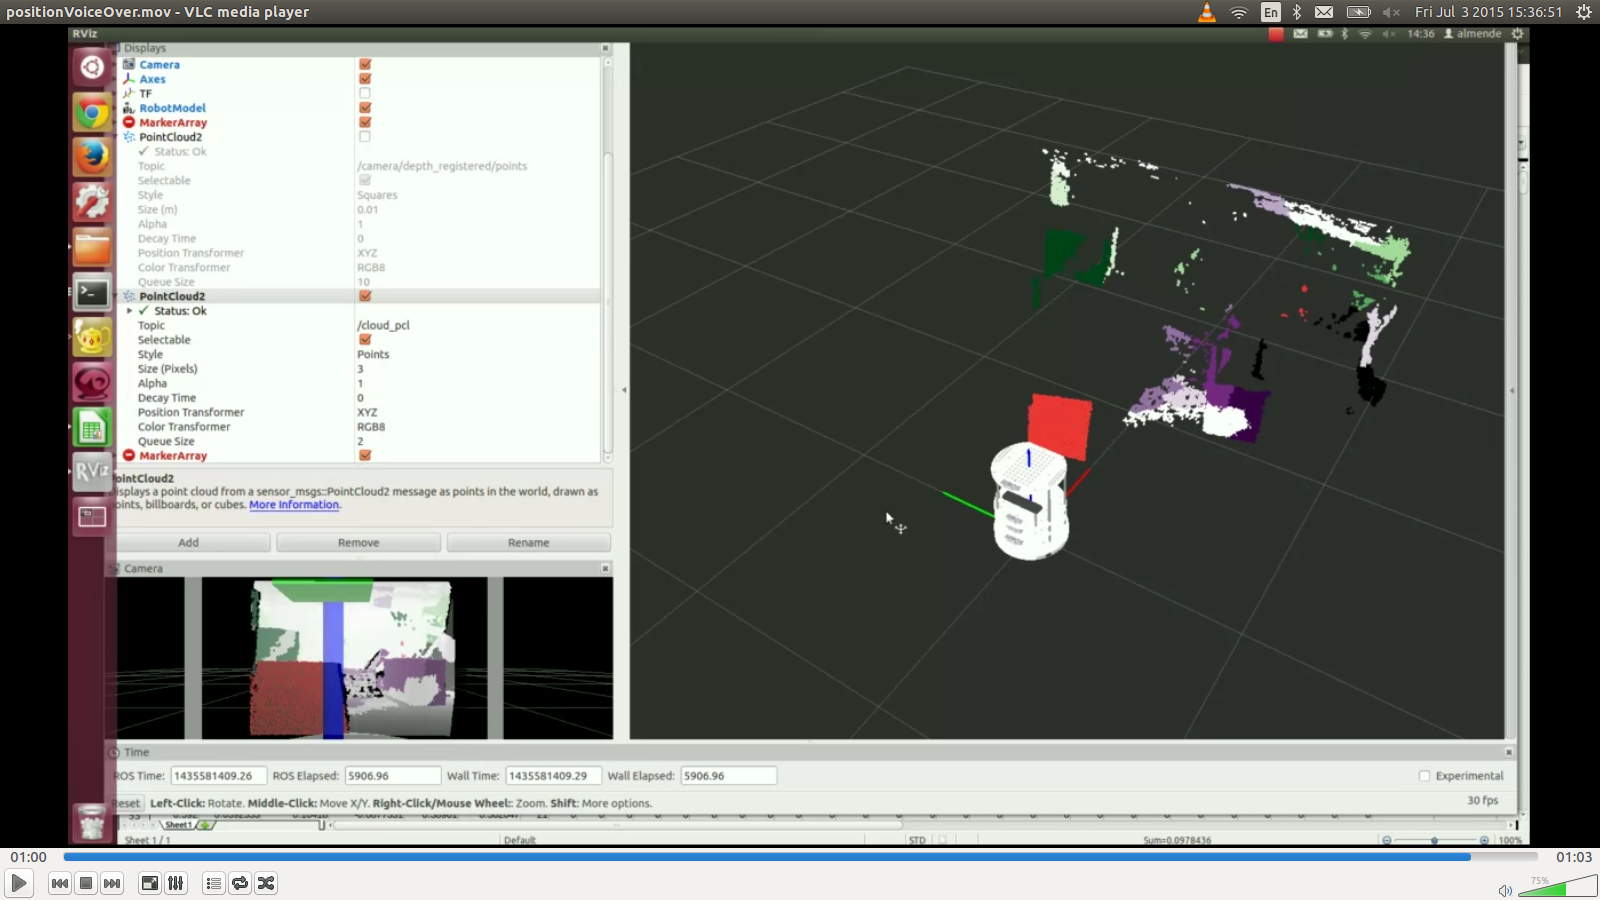
\includegraphics[width=.3\textwidth]{posBound2} \\
            (c) Folder initial  & (d) Folder moved \\[6pt]
        \end{tabular}
        \caption{Expresiveness \& decision bounds}
        \label{pip:bounds}
    \end{wrapfigure}

    In Fig.\ref{pip:bounds}(a) the yellow folder allong with some of its environment to the left are being assigned to landmark with id 7383. The folder is then removed and a blue trashcan is put in its place. The folder and the trashcan are similar in size and due to that their Gaussian counterparts will not have large distances. Their main difference lies in the color signature they carry. Since the distance in their color is substantial, a new landmark with id 7412 is created to capture the change in the signature of the environment at that place of the map. The different landmark assigned to the cluster can be seen in Fig.\ref{pip:bounds}(b). In Fig.\ref{pip:bounds}(c) and(d) the positional decision boundary is displayed. In the initial position as shown in Fig.\ref{pip:bounds}(c) the yellow folder is assigned to the green landmark of the cloud. As the object is moved a different position in the cloud, it is being assigned to a different cluster. The reason the cluster is assigned to multiple landmarks is due to the fact that the folder is decomposed to several clusters and each one of them is being assigned to a different part of the cloud with respect to their position. This can be seen in Fig.\ref{pip:bounds}(c) where the bottom left of the folder is being assigned to the red cluster. Parameter tweaking is possible but the purpose of a general pipeline is to use as little parameter tweaking as possible so that the method is general and can easily be applied to a different scenarios.


    The exponential part of the distribution is responsible for the angle signature elements within a cluster have. Practically, having a large amount of different angle distributions in a single cluster leads to objects that have texture and their surface is not smooth. Having a very strict limit in the angle distribution can lead to very small clusters and subsequently to a high amount of landmarks within the data. Using the data from the kinect camera, angle distributions are sensitive to noise that is found in parts of the cloud that are near the end of Kinect sensor's range. Practical evaluation has shown that using an angle limit that is close to the average distance between angle signatures produces stable results and reasonably sized landmarks in the cloud.

    \subsection{EKF-slam experiments}

    Finally, the pipeline was used in real life scenarios as a sensor model in a Landmark based EKF slam algorithm and was tested in its precision and memory requirements. In Fig.\ref{slam} an end result of a slam session using the pipeline as a sensor model is shown. As the robot progresses through the environment, the EKF module requests from the sensor model to observe what landmarks are currently detected given the current cloud readings and the existing Landmark database. The pipeline follows the procedure defined in the general pipeline section and returns the landmarks currently detected. The end results shows the amount of landmarks the method requires in order to map a medium sized room. Each sphere represents an environment signature at that specific point the same way it was shown in the simple datasets sections. If the decision layer is chosen to be very strict the number of landmarks the algorithm outputs will increase, and the environment will be represented in more detail. It is important to notice that a strict decision layer must be handled with care as it can lead to a pipeline that continuously adds new landmarks making the sensor module non-converging.


    \begin{wrapfigure}{l}{0.4\textwidth}
        \begin{tabular}{c}
            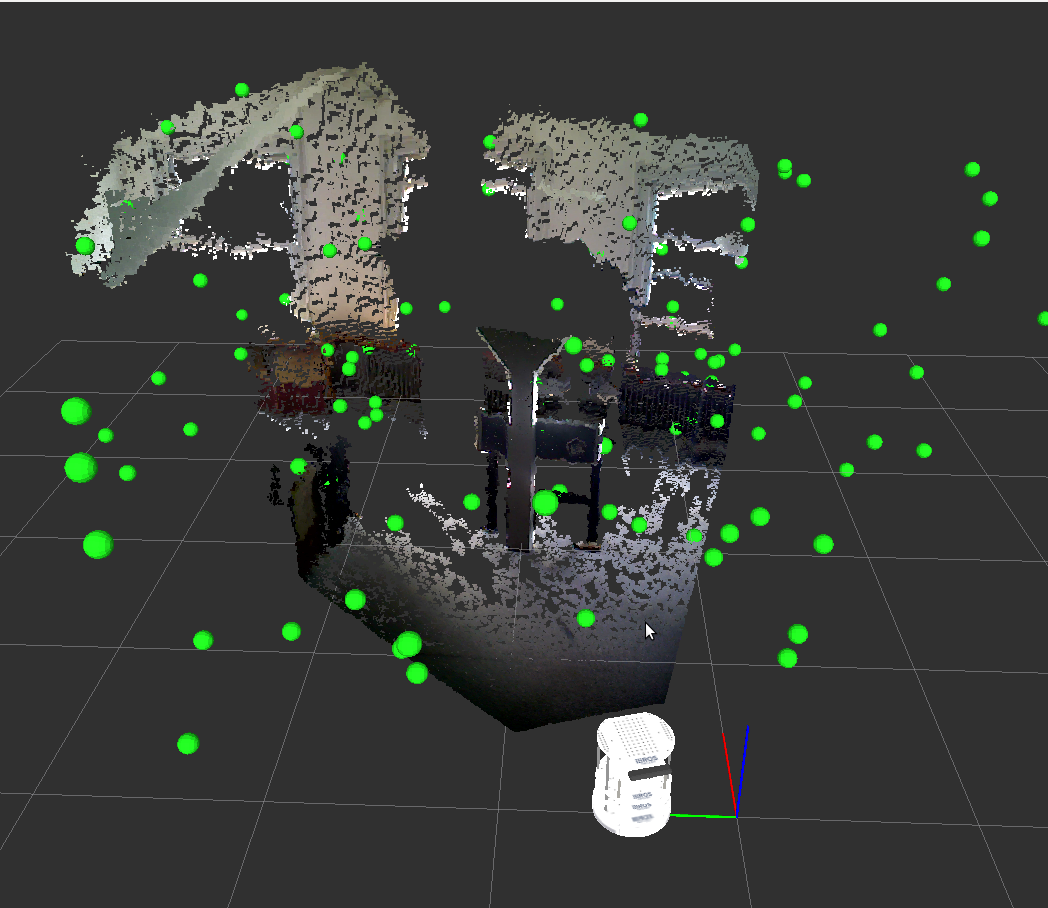
\includegraphics[width=.353\textwidth]{slam110landmarks2} \\
            (a) Slam session \\
            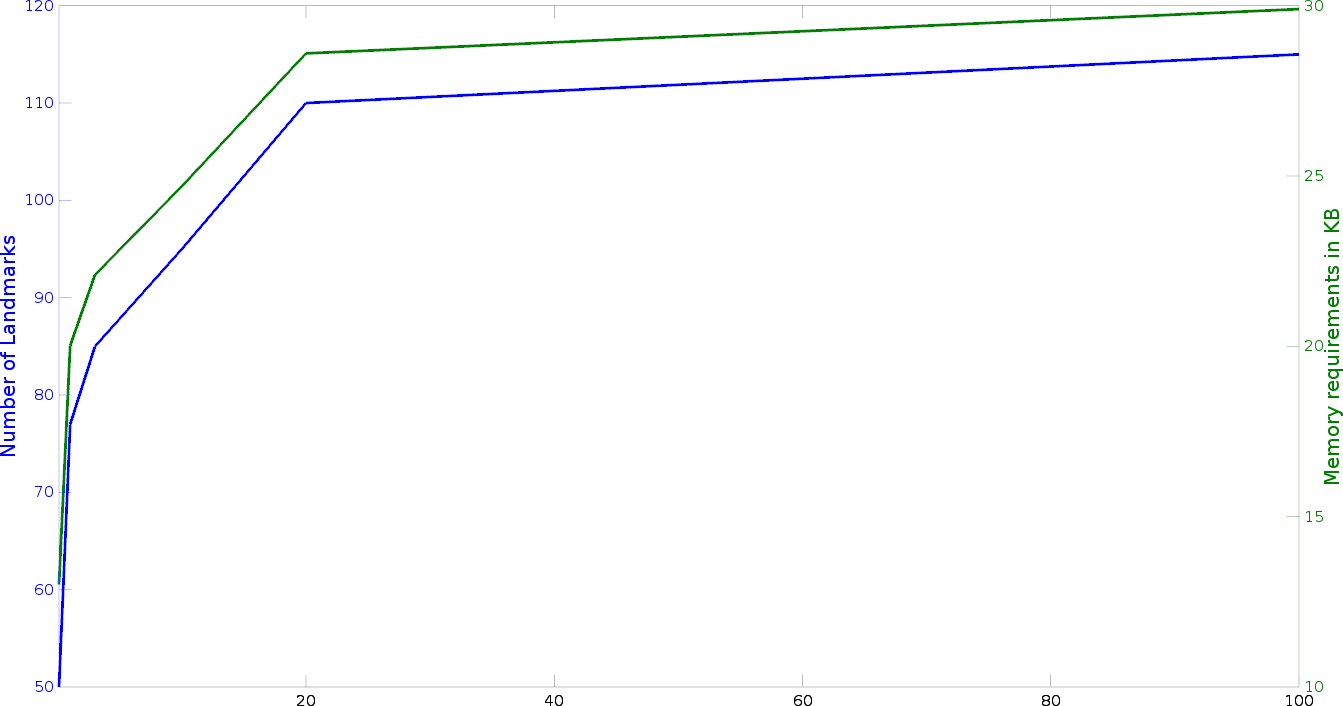
\includegraphics[width=.353\textwidth]{memoryRequirements} \\
            (b) Memory requirements \\[6pt]
        \end{tabular}
        \caption{SLAM session and memory requirements}
        \label{slam}
    \end{wrapfigure}

    The compression that method introduces is not directly observable from the figure. As the environment is being reduced from a cloud to a landmarks, the memory needs change from using point clouds to using the landmarks extracted in those clouds. Since every landmark represents a signature of the environment at this particular point, the compression is done by reducing a high amount of points to that specific signature. The number of parameters needed to define the three distributions in the signature is all the information this method requires and hence the memory gains are substantial. The expresiveness of the distributions greatly affects the objects as well as object shapes that could be represented. Finally it is always possible to extend the method presented by adding new features and new priors to those features.


    \subsection{Memory requirements}

    The memory requirements of the method is related to the Dirichlet strength parameter $\alpha$ of the sampler. As the $\alpha$ parameter increases, the sampler will output more clusters on every iteration. The higher amount the of cluster will result a higher amount of landmarks and, consequently, in larger memory requirements in the method. Fig.\ref{slam}(b) shows memory requirements as a function of strength parameter alpha.

    As it can be seen, the number of landmarks follows the logarithmic trend of the Dirichlet prior in relation to $\alpha$. Constantly increasing the alpha value will not make the algorithm follow the logarithmic trend indefinitely. That is due to the fact that despite the alpha increase, the decision layer has an upper bound to the number of landmarks it can have and will eventually saturate. It must also be noted that as the alpha parameter is set to higher numbers, the sampler outputs more clusters making it a more accurate environment descriptor, but also takes more time, making it non feasible to use in real time scenarios. Values of alpha between 0 and 10 provide a robust and fast enough sampler that can be used in online mapping scenarios.

    \subsection{Limits of the method}

    Limits of the method exist in relation to the two basic layers of the pipeline. The clustering layer and the decision making.

    \subsubsection{Clustering layer}
    \begin{wrapfigure}{l}{.6\textwidth}
        \begin{tabular}{cc}
            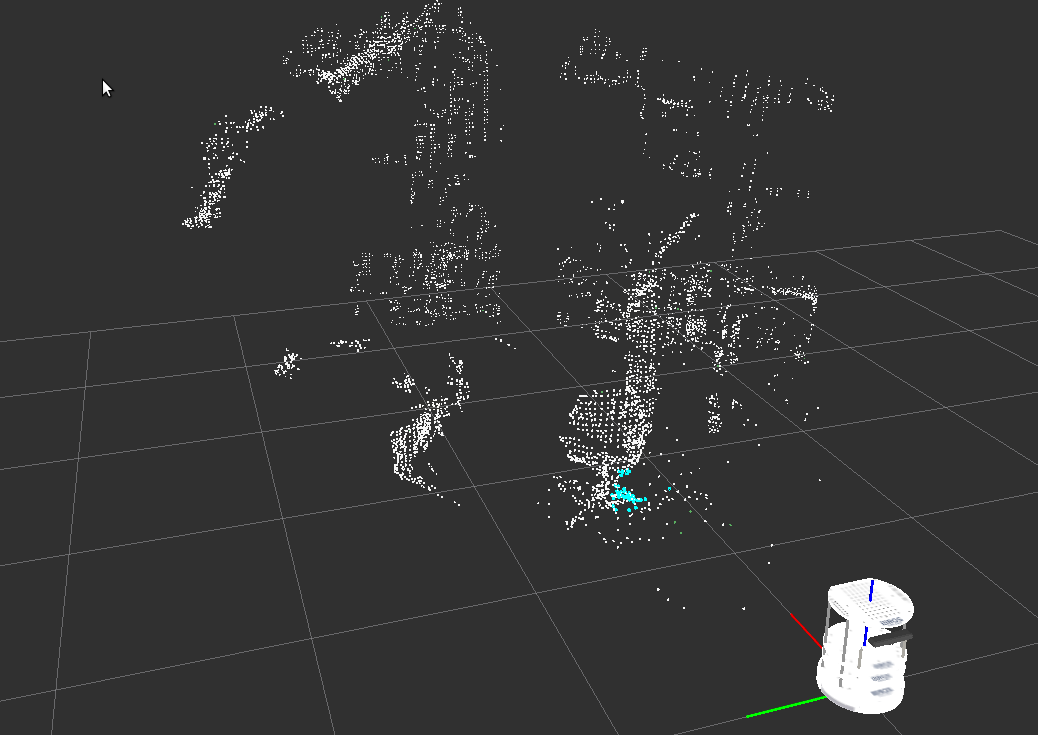
\includegraphics[width=.26\textwidth]{singlecluster} &  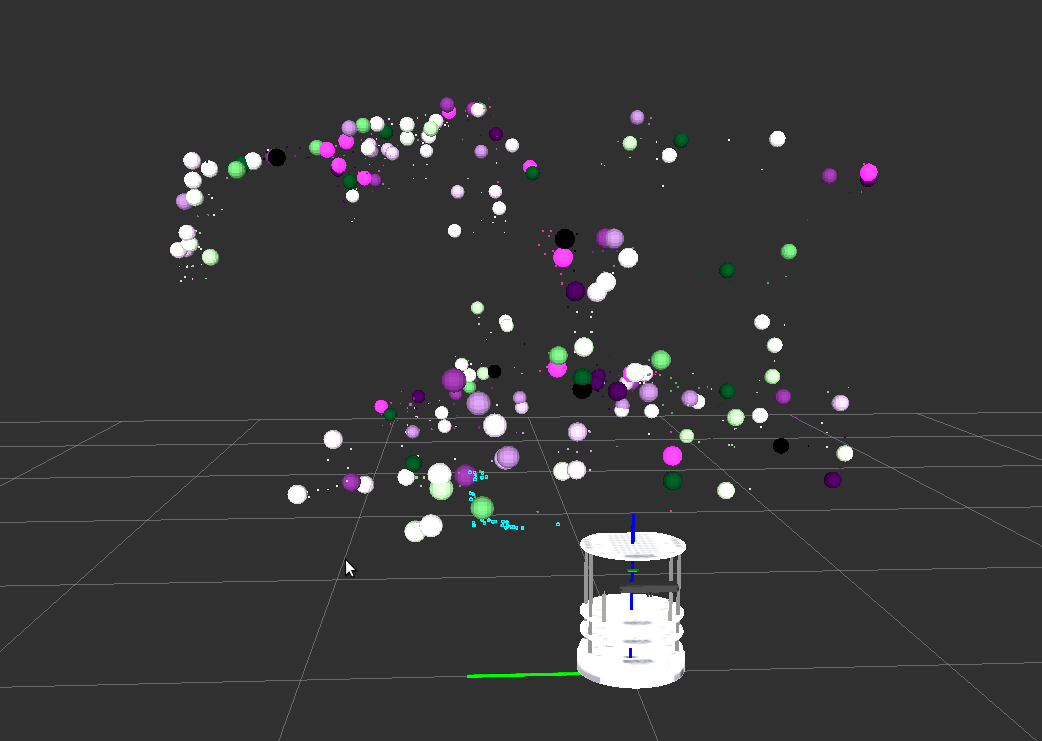
\includegraphics[width=.26\textwidth]{onlyclusters2} \\
            (a) Low $\alpha$ & (b) High $\alpha$ pipeline\\
        \end{tabular}
        \caption{Pipeline fail cases.}
        \label{pip:limits}
    \end{wrapfigure}

    An important limit of the pipeline exists with respect to the Dirichlet hyper-parameter $\alpha$. During the clustering, choosing a correct value for the hyper-parameter $\alpha$ is very important in order to have optimal results. Having sampler run with a very low $\alpha$ can lead to the whole cloud being assigned a single cluster. Having every point in the cloud being part of the same cluster leads to a a significant amount of information loss as no environment specific information are incorporated to the cloud. Fig.[\ref{pip:limits}](a) shows the behaviour of the sampler for $\alpha$ values lower than 1. 



    On the other hand, having a very large $\alpha$ can lead to a very large amount of clusters being output by the sampler every time. That can lead to a non-converging pipeline since every time a new landmark that does not fit the landmark database is output. This leads to many small clusters each containing small number of points each. Furthermore, having a high value in the hyperparameter leads to a slower sampling procedure since the complexity of the sampler is $O(TKLSN)$ where $K$ is the number of clusters. Fig.[\ref{pcl:kl}](b) displays the behavior of the sampler for very large values $\alpha$. The spheres represent landmarks and it can be seen that most of the points in the environment are considered individually clusters.


    \subsubsection{Decision layer}

    The restrictions imposed by the decision layer are straightforward due to the constant nature of the decision process. Taking very small distances in the distance threshold operation can lead to pipeline that continuously adds new landmarks to the database. An example is shown in Fig.~\ref{pip:expo} where limiting the landmark matching operation to very small exponential distances, leads to a cloud where objects are decomposed to a lot entitites.

    \begin{wrapfigure}{l}{.45\textwidth}
        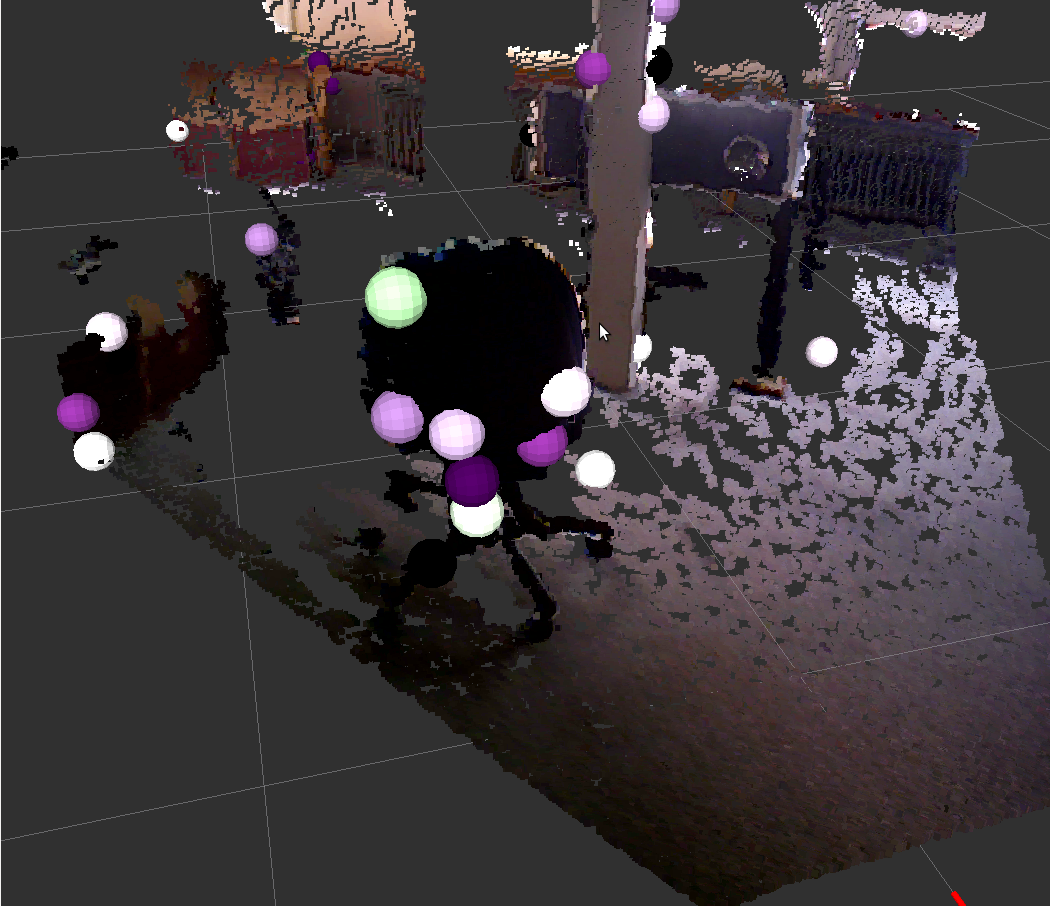
\includegraphics[width=.4\textwidth]{monsterchair} \\
        \caption{Strict exponential limit}
        \label{pip:expo}
    \end{wrapfigure}

    Object decomposition is even more intense when camera movement is involved due to the different angles. Finally, since the number of landmarks is also a function of noise, areas of the cloud that are near the maximum range of the sensor can lead to different landmarks added frequently.
    %------------------------------------------------

    \section{Conclusion and future work}
    \label{sec:discussion}

    In this paper a novel method for cloud representation by using non-parametric Bayesian tools was introduced. By reducing parts of the environment to distribution signatures, a large amount of compression is provided making the method highly suitable to target long term slam problems; the expresiveness of the representation is enough to perform slam and is robust even in the noisy parts of the environment. The strengths and weaknesses of the method were presented and an application on how this method could be used to tackle the compression problem of long term slam were given.

    There is a number of directions which could be explored to improve the method. Choosing more complex environment representations could increase the expresive strength of the sampler making it easier to represent with higher precision more complex structures. Also, a hierarchical clustering approach would be an interesting extension since it would both have the ability to capture the structure in a top-down maner and as well as handle the dynamic component that long term slam problems introduce. Furthermore, having a more complex decision layer would also increase the robustness of the method making it able to handle more complex environment structures and more expresive landmarks. Finally, those additions could help lift the dynamic environment restrictions that were defined in Walcotts PhD thesis and make the pipeline tackle in a fully Bayesian way the implications of life-long slam.

    %----------------------------------------------------------------------------------------
    %	REFERENCE LIST
    %----------------------------------------------------------------------------------------

    \begin{thebibliography}{99} % Bibliography - this is intentionally simple in this template

        \bibitem{probRobs}
            \newblock Thrun, S. (2002). Probabilistic robotics. Communications of the ACM, 45(3), 52-57.


        \bibitem{ekf} \newblock Bailey, T., Nieto, J., Guivant, J., Stevens, M., \& Nebot, E. (2006, October). Consistency of the EKF-slam algorithm. In Intelligent Robots and Systems, 2006 IEEE/RSJ International Conference on (pp. 3562-3568). IEEE.  

        \bibitem{liflonglearning}
            \newblock Thrun, S., \& Mitchell, T. M. (1995). Lifelong robot learning. The Biology and Technology of Intelligent Autonomous Agents, 165-196.

        \bibitem{lifelongmaps}
            \newblock Konolige, K., \& Bowman, J. (2009, October). Towards lifelong visual maps. In Intelligent Robots and Systems, 2009. IROS 2009. IEEE/RSJ International Conference on (pp. 1156-1163). IEEE.

        \bibitem{aishalong}
            \newblock Walcott, A. (2011). Long-term robot mapping in dynamic environments. 

        \bibitem{pcl}
            \newblock{Rusu, R. B., \& Cousins, S. (2011, May). 3d is here: Point cloud library (pcl). In Robotics and Automation (ICRA), 2011 IEEE International Conference on (pp. 1-4). IEEE.}


        \bibitem{slam++}
            \newblock Salas-Moreno, R. F., Newcombe, R. A., Strasdat, H., Kelly, P. H., \& Davison, A. J. (2013, June). Slam++: Simultaneous localisation and mapping at the level of objects. In Computer Vision and Pattern Recognition (CVPR), 2013 IEEE Conference on (pp. 1352-1359). IEEE.

        \bibitem{objslam}
            \newblock Selvatici, A. H., \& Costa, A. H. (2008). Object-based visual slam: How object identity informs geometry.

        \bibitem{objectpointslam}
            \newblock Choudhary, S., Trevor, A. J., Christensen, H. I., \& Dellaert, F. (2014, September). slam with object discovery, modeling and mapping. In Intelligent Robots and Systems (IROS 2014), 2014 IEEE/RSJ International Conference on (pp. 1018-1025). IEEE.

        \bibitem{objectDisc}
            \newblock Koo, S., Lee, D., \& Kwon, D. S. (2014, September). Unsupervised object individuation from RGB-D image sequences. In Intelligent Robots and Systems (IROS 2014), 2014 IEEE/RSJ International Conference on (pp. 4450-4457). IEEE.

        \bibitem{fpfh}
            \newblock{Fast point feature histogram.Rusu, R. B., Blodow, N., \& Beetz, M. (2009, May). Fast point feature histograms (FPFH) for 3D registration. In Robotics and Automation, 2009. ICRA'09. IEEE International Conference on (pp. 3212-3217). IEEE.}

        \bibitem{segOverview}
            \newblock {Rabbani, T., van den Heuvel, F., \& Vosselmann, G. (2006). Segmentation of point clouds using smoothness constraint. International Archives of Photogrammetry, Remote Sensing and Spatial Information Sciences, 36(5), 248-253.}

        \bibitem{nonParam}
            \newblock{Wainwright, M. J., \& Jordan, M. I. (2008). Graphical models, exponential families, and variational inference. Foundations and Trends in Machine Learning, 1(1-2), 1-305.}
            ``
        \bibitem{omnimaper}
            \newblock{A.Trevor,  J.Rogers, and  H.Christensen.  Omnimapper:  A  modular multimodal  mapping  framework.   In IEEE  International  Conference on Robotics and Automation (ICRA), 2014}

        \bibitem{pointSeg}
            \newblock Trevor, A. J., Gedikli, S., Rusu, R. B., \& Christensen, H. I. (2013). Efficient organized point cloud segmentation with connected components. Semantic Perception Mapping and Exploration
        \bibitem{planarSeg}
            \newblock Unnikrishnan, R., \& Hebert, M. (2003, October). Robust extraction of multiple structures from non-uniformly sampled data. In Intelligent Robots and Systems, 2003. Proceedings. 2004 IEEE/RSJ International Conference on IEEE. 

        \bibitem{planarSeg2}
            \newblock Rabbani, T., van den Heuvel, F., \& Vosselmann, G. (2006). Segmentation of point clouds using smoothness constraint. International Archives of Photogrammetry, Remote Sensing and Spatial Information Sciences, 36(5), 248-253.

        \bibitem{smartSeg}
            \newblock Triebel, R., Shin, J., \& Siegwart, R. (2010, June). Segmentation and unsupervised part-based discovery of repetitive objects. In Robotics: Science and Systems (Vol. 2).

        \bibitem{smcddp}
            \newblock Neiswanger, W., Wood, F., \& Xing, E. (2014, August). The dependent dirichlet process mixture of objects for detection-free tracking and object modeling. In Proceedings of the Seventeenth International Conference on Artificial Intelligence and Statistics (pp. 660-668).

        \bibitem{corresp:first}
            \newblock Cree, M. J., Jefferies, M. E., \& Baker, J. T. Using 3D Visual Landmarks to Solve the Correspondence Problem in Simultaneous Localisation and Mapping.

        \bibitem{corres:sec}
            \newblock Lowe, D. G. (2004). Distinctive image features from scale-invariant keypoints. International journal of computer vision, 60(2), 91-110.

        \bibitem{corres:three}
            \newblock Lamon, P., Tapus, A., Glauser, E., Tomatis, N., \& Siegwart, R. (2003, October). Environmental modeling with fingerprint sequences for topological global localization. In Intelligent Robots and Systems, 2003. Proceedings. 2003 IEEE/RSJ International Conference on IEEE.


        \bibitem{corres:four}
            \newblock Sehgal, A., Cernea, D., \& Makaveeva, M. (2010). Real-time scale invariant 3D range point cloud registration. In Image Analysis and Recognition (pp. 220-229). Springer Berlin Heidelberg.

        \bibitem{bayes:neal}
            \newblock Neal, R. M. (2000). Markov chain sampling methods for Dirichlet process mixture models. Journal of computational and graphical statistics, 9(2), 249-265.

        \bibitem{bayes:jordan}
            \newblock Blei, D. M., \& Jordan, M. I. (2006). Variational inference for Dirichlet process mixtures. Bayesian analysis, 1(1), 121-143.

        \bibitem{slam}
            \newblock{Montemerlo, M., Thrun, S., Koller, D., \& Wegbreit, B. (2002). Fastslam: A factored solution to the simultaneous localization and mapping problem. AAAI/IAAI, 593-598.}

        \bibitem{bayes:smc}
            \newblock Doucet, A., De Freitas, N., \& Gordon, N. (2001). An introduction to sequential Monte Carlo methods (pp. 3-14). Springer New York.

        \bibitem{antoniak}
            \newblock{Charles E Antoniak,Mixtures of dirichlet processes with applications to bayesian nonparametric problems, The annals of statistics (1974), 1152–1174}

        \bibitem{caron}
            \newblock{F. Caron, M. Davy, and A. Doucet, Generalized Polya urn for time-varying Dirichlet process mixtures, 23rd Conference on
                Uncertainty in Artificial Intelligence (UAI’2007), Vancouver,
            Canada, July 2007, 2007}

        \bibitem{compendium}
            \newblock{Fink, D. (1997). A compendium of conjugate priors.}

        \bibitem{smc:theory}
            \newblock{Ülker, Y., Günsel, B., \& Cemgil, A. T. (2010). Sequential Monte Carlo samplers for Dirichlet process mixtures. In International Conference on Artificial Intelligence and Statistics}

        \bibitem{doucet}
            \newblock{Del Moral, P., Doucet, A., \& Jasra, A. (2006). Sequential monte carlo samplers. Journal of the Royal Statistical Society: Series B (Statistical Methodology), 68(3), 411-436.}

        \bibitem{RANSAC}
            \newblock{Meer, P., Mintz, D., Rosenfeld, A., \& Kim, D. Y. (1991). Robust regression methods for computer vision: A review. International journal of computer vision, 6(1), 59-70.}

    \end{thebibliography}

    %----------------------------------------------------------------------------------------


    \end{document}
